% ============================================================================
% Section 1 -- introduction. Rewritten 2026-09-27 against Ben's comments on the
% first five pages: define or drop every symbol, do not open on the negative,
% say why per-request granularity matters, and use his contribution framing.
% Compressed the same day to ~1.25pp -- the front of the paper was pushing the
% evaluation to p10.
% ============================================================================

\section{Introduction}
\label{sec:intro}

A GPU serving LLM decode is mostly idle. Generating one token for a batch reads every
model weight and every resident KV byte with almost no arithmetic per byte, so the
arithmetic units run at single-digit utilization while the memory system saturates.
What stops the server batching more requests is not compute: the KV cache has
exhausted device memory. A trace-driven study reaches the same conclusion from the
workload side, finding device memory capacity rather than token budget to be what
binds~\cite{bottlenecks}.

The machine has more memory than the GPU's. A Grace-Hopper
node~\cite{gracehopper} pairs 96\,GB of HBM with hundreds of gigabytes of host DRAM,
and NVLink-C2C connects them at 450\,GB/s per direction --- the commonly quoted 900
is bidirectional, where a KV stream is not. At that rate the KV a decoding request
needs can cross the link inside the window during which the GPU is reading its own
weights and wants nothing from the link. Host DRAM stops being a place to park idle
requests and becomes usable memory for running ones.

\paragraph{Two memories, managed as one.} This paper builds a heterogeneous memory
system for LLM decode: HBM and host DRAM managed as a single KV store, with each
request assigned to a tier. A \textbf{device-tier} request behaves as in stock vLLM;
a \textbf{host-tier} request holds no device blocks at all, its KV living in host
memory and each layer's bytes streamed across the link just before that layer's
attention reads them, into a small buffer reused across all layers --- four buffers
for a 64-layer model, about 6\% of the device memory a resident request needs. Both
tiers are rows of the same batch in one forward pass, so the weights are read once
however the batch is split. The target throughout is a decode node in a
prefill/decode-disaggregated deployment~\cite{distserve,splitwise,mooncake}, where a
request arrives with its KV already computed --- the assumption that makes a
host-tier request \emph{additive} rather than merely relocated
(\S\ref{sec:background:pd}).

\paragraph{Why choose per request.} Existing systems vary \emph{how much} KV sits on
the host and never \emph{whose}. vLLM~\cite{vllm} and SGLang~\cite{sglang} keep all
of it in HBM and make requests wait; DirectKV~\cite{directkv} keeps all of it on the
host, always, which is why it needs no memory management at all. Pie~\cite{pie}, the
closest prior work, genuinely uses both memories --- $m$ of a model's $n$ layers on
the host --- but that split applies to every request identically
(\S\ref{sec:related}). Choosing per request buys three things a uniform fraction
cannot: capacity freed in \emph{whole} requests rather than in proportion, movement
once per request at a moment the scheduler picks rather than once per layer per
token, and link bandwidth spent only on the requests we select. And neither endpoint
is optimal for a reason visible without measurement --- each leaves one KV path
entirely idle, where a system placing some requests in each reads from both and its
batch is bounded by the sum: for Qwen2.5-32B fp16 at 8K on a GH200-96, 18 against 12
all-HBM and 6 all-host (Table~\ref{tab:endpoints}).

\paragraph{When does a second tier pay?} Before building one we ask when it is
worth having, and the answer is narrow enough to be useful. Two consequences of the
capacity model run against intuition: long context does \emph{not} help, shrinking
the resident and affordable host cohorts in the same proportion, and the value of a
second tier tracks \textbf{how much of memory the weights consumed} rather than
model size --- sharpest in that the \emph{same model at two weight precisions} lands
at two different points on the curve. Capacity is not throughput, though, and the
gap is where this paper spends its effort: charging the host path's fixed per-step
cost as well as its per-request cost gives a second condition that binds harder than
the latency gate (\S\ref{sec:model:omits}).

\paragraph{Contributions.}
\begin{enumerate}\itemsep2pt
\item \textbf{A heterogeneous KV memory manager} (\S\ref{sec:design}): HBM and host
      DRAM as one store, in which a host-tier request holds no device blocks
      \emph{while it is generating}, so tiered requests are additive rather than
      substitutional. This is the distinction from every system that tiers KV at
      request granularity: they \emph{take turns}, pausing a request while its KV
      sits in host memory, so the running batch's KV is always resident. Ours is
      decoded from host memory in the same forward pass as the resident cohort
      (\S\ref{sec:related}).
\item \textbf{A capacity model that picks a configuration from a profile}
      (\S\ref{sec:model}): given measured bandwidths and the host path's two costs
      it returns the host cohort that maximises decode throughput, and says when
      that cohort is zero.
\item \textbf{An admission controller in vLLM} (\S\ref{sec:design:admission}): the
      host cohort sized at runtime from the rider-free step time and the achieved
      link bandwidth, not from a configured offload fraction.
\item \textbf{A working implementation, and a measured account of what it costs}
      (\S\ref{sec:eval}). The mechanism itself is demonstrated rather than
      projected: six times the concurrency from the same KV pool, output
      token-identical to the unmodified engine. The interconnect we have is too slow
      for that capacity to convert into throughput --- which the model predicts
      before we measure it --- so the cost decomposition is what carries the
      projection --- whose inputs are anchored to published Grace-Hopper
      measurements\ifarxiv, consolidated in \S\ref{app:validation}\fi.
\end{enumerate}

\begin{figure}[t]
\centering
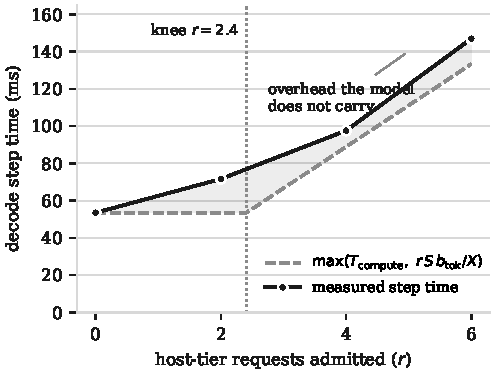
\includegraphics[width=\columnwidth]{figs/f6.pdf}
\caption{The cost of a host-tier request, and the knee that organises it. Below the
knee the transfer fits inside a step and hides \emph{completely}; above it the step
\emph{is} the transfer, and fitting one line across the boundary --- which we did,
and report in \S\ref{sec:eval:cost} --- overstates the per-rider slope while
understating the fixed cost, from that single cause. Measured strictly below the
knee the law is affine: a \emph{fixed} $3.4$\,ms per step at 64 layers plus
$0.52$\,ms per request. A faster link moves the knee right, which is the whole of
what it buys; it does not shrink either term. Qwen2.5-32B, 2048 context, 16
residents, A100/PCIe at 25.1\,GB/s, 3 repeats under 1\% spread.}
% src: paper/data/rider_cost_phase0.json @ fb7e9db2a
\label{fig:costcurve}
\end{figure}

\paragraph{What it costs, and why PCIe cannot pay.}
Figure~\ref{fig:costcurve} is the measurement the rest of the paper turns on. Two
host-tier requests grow a $54.1$\,ms step to $70.8$, and the curve bends where the
aggregate transfer stops fitting inside a step. That bend --- the \emph{knee} --- is
the structure that matters, and locating it changed our reading of everything else:
measured below it, a rider's transfer hides completely and the per-request cost is
$0.61$\,ms of exposed launch work carrying no bandwidth term at all
(\S\ref{sec:eval:cost}). What a faster interconnect buys is therefore not a cheaper
rider but a higher knee, and so more riders at the same price.

That settles the PCIe case, since a larger batch pays only if the step grows by
less: the link affords two host-tier requests on sixteen residents, a batch of
$1.13\times$ against a step growing $1.31\times$, for a product of $0.86\times$.
The mechanism itself we confirm independently of its economics, raising peak
concurrency against a fixed KV pool from 8 to 48 (\S\ref{sec:eval:capacity}).
% src: paper/data/preload_capacity.json @ f3df05bdb
On a coherent link the model projects gains for all four configurations, from
$\times 1.04$ to $\times 1.37$, ordered by how much of the device the weights
consumed. Two things decide whether those are collected: a fixed per-step cost,
which we cut by $74\%$ and then account for, and the integrality of the rider
cohort --- a budget admitting $1.89$ riders admits one, so the achievable gain is a
sawtooth in context and a $5\%$ change in it is worth $18\%$
(\S\ref{sec:model:knee}).
